%\algnewcommand{\IfNDebug}[1]{#1}
%\algnewcommand{\IfNDebug}[1]{}

\newcommand{\varStartG}{\ensuremath{\AlgVar{start}_G}}
\newcommand{\varEndG}{\ensuremath{\AlgVar{end}_G}}
\newcommand{\varStartH}{\ensuremath{\AlgVar{start}_H}}
\newcommand{\varEndH}{\ensuremath{\AlgVar{end}_H}}
\newcommand{\varActive}{\ensuremath{\AlgVar{active}}}
\newcommand{\varSplitting}{\ensuremath{\AlgVar{splitting}}}
\newcommand{\varPrev}{\ensuremath{\AlgVar{prev}}}
\newcommand{\varNext}{\ensuremath{\AlgVar{next}}}
\newcommand{\labelClass}{\ensuremath{\AlgVar{labelClass}}}
\newcommand{\vertexPtr}{\ensuremath{\AlgVar{vertexPtr}}}
\newcommand{\calLC}{\ensuremath{\mathcal{LC}}}
\newcommand{\LC}{\ensuremath{\AlgVar{LC}}}
\newcommand{\Gptrs}{\ensuremath{\AlgVar{Gptrs}}}
\newcommand{\Hptrs}{\ensuremath{\AlgVar{Hptrs}}}
\newcommand{\Garray}{\ensuremath{A_G}}
\newcommand{\Harray}{\ensuremath{A_H}}

\chapter{McSplit-SI: An algorithm for the induced subgraph isomorphism problem}
\label{c:mcsplit-si}

\section{Introduction}

In the induced subgraph isomorphism problem, we seek an induced copy of pattern graph $G$ in target graph $H$. This is a special case of the decision version of maximum common induced subgraph in which we require the common subgraph to contain all of graph $G$'s vertices.

The \McSplit\ algorithm may be trivially modified to solve the induced subgraph isomorphism problem. Rather than calculating an upper bound at each search node, we simply backtrack when the $G$-set of any label class is larger than the corresponding $H$-set, since by the pigeonhole principle this implies that we cannot map each pattern-graph vertex to a target-graph vertex.

While \McSplit\ is well suited to the small (tens of vertices), relatively dense pattern and target graphs that are typical of maximum common subgraph instances, it has two disadvantages for large (hundreds or thousands of vertices), sparse graphs that appear in benchmark instances for subgraph isomorphism.  The first disadvantage relates to space: $b(n_G^2 + n_H^2)$ space is needed to store the adjacency matrices, where $b$ is the memory size of a boolean variable.\footnote{We could switch to a more space-efficient representation such as hash-sets of neighbours which would still permit amortized constant time adjacency tests in the algorithm's partitioning step, but this would slow down the algorithm significantly.}  The second disadvantage relates to time: during the partitioning step, the \McSplit\ algorithm iterates over all of the vertices in each label class, which often requires checking close to $n_G + n_H$ adjacency-matrix elements each time the partitioning procedure is carried out.

\begin{figure}[htb]
    \centering
    \includegraphics*[width=0.6\textwidth]{14b-mcsplit-induced-si/density-chart/plots/n-density-pdf}
    \caption{Number of vertices and density (log scale) for each target graph in the benchmark set
    of $14,621$ subgraph isomorphism decision instances.}
    \label{figure:si-targets-n-density}
\end{figure}

\Cref{figure:si-targets-n-density} shows vertex count and density for the target graphs of the benchmark instances
that we will use in this chapter.  Of the entire benchmark set, $76\%$ of pattern graphs have density less than $0.01$.  Thus, it would
greatly improve our \McSplit\ algorithm for subgraph isomorphism on these and similar instances if we could reduce the time complexity of the partitioning
step from $O(n_G + n_H)$ to $O(|N(v)| + |N(w)|)$, where $(v,w)$ is the most-recently made mapping of a pattern vertex to a target
vertex.  In this chapter we introduce this improved algorithm, which we call \McSplit-SI.

\section{The label class object}

In the basic version of the \McSplit\ algorithm that was described in
\Cref{c:mcsplit-i-undirected}, the label class objects at each level of the search tree are stored
contiguously in an array, and each object representing
a label class $\langle S_G, S_H \rangle$ requires only four indices or pointers: to the start and
end of the array slices that contain $S_G$ and $S_H$.
To enable partitioning in $O(|N(v)| + |N(w)|)$ time, \McSplit-SI
requires a more elaborate label-class object, and stores the objects in a doubly-linked list which is modified
when partitioning domains and restored on backtracking.

\Cref{tab:mcsplit-si-object} lists the member variables of a label class object.
The first two members are $\AlgVar{prev}$ and $\AlgVar{next}$ pointers, which
allow the set of label classes to be jointed together as a doubly-linked list.
These pointers are useful not only for iterating over the list but also
for restoring deleted elements when backtracking, as we will discuss later in the chapter.

The next four members of the object play the same role as the four indices used in \McSplit's
simpler label class object: they point to the ranges in the permuations of $V(G)$ and $V(H)$ that
contain $S_G$ and $S_H$.

Finally, we have two boolean flags, $\varActive$ and $\varSplitting$.  The first flag
records whether the label class object is currently in the list of label classes.  (Inactive
label classes have been deleted, but are maintained in memory so that they can be restored
when backtracking.)  The second flag is used temporarily during the partitioning step
to record which label class have been partitioned.

\begin{table}[htb]
\centering
\footnotesize
 \begin{tabular}{p{0.13\linewidth} p{0.2\linewidth} p{0.5\linewidth}}
 \toprule
    Name & Type & Description \\ [0.5ex]
 \midrule
    $\AlgVar{prev}$ & Pointer to Label Class & The previous label class in the doubly-linked list of all label classes \\
    \rule{0pt}{2.3ex}$\AlgVar{next}$ & Pointer to Label Class & The next label class in the doubly-linked list of all label classes \\
    \rule{0pt}{2.3ex}\varStartG & Pointer to Integer & Pointer to the first vertex of the $G$-set\\
    \rule{0pt}{2.3ex}\varEndG & Pointer to Integer & Pointer to one element past the last vertex of the $G$-set\\
    \rule{0pt}{2.3ex}\varStartH & Pointer to Integer & Pointer to the first vertex of the $H$-set\\
    \rule{0pt}{2.3ex}\varEndH & Pointer to Integer & Pointer to one element past the last vertex of the $H$-set\\
    \rule{0pt}{2.3ex}$\AlgVar{active}$ & Boolean & Is this label class in the doubly linked list? \\
    \rule{0pt}{2.3ex}$\AlgVar{splitting}$ & Boolean & Is this label class being split? \\
 \bottomrule
\end{tabular}
\caption{The member variables of \McSplit-SI label class object}
\label{tab:mcsplit-si-object}
\end{table}

The collection of data structures used by \McSplit-SI to represent the set of active label
classes has three components.  The first of these is the the doubly-linked list of label
class objects that we have described; we refer to this as \calLC.  The second 
component is the pair of arrays that store partitions of $V(G)$ and $V(H)$ that are pointed
to by each label class object.   We call these arrays $\Garray$ and $\Harray$.

The final component of our collection of data structures contains two arrays, $\Gptrs$
and $\Hptrs$.  These contain
an object for each vertex $v$ of $G$ and $H$ respectively.  Each object contains two pointers.
The first pointer of $\Gptrs[v]$ points to the position in $\Garray$ at which $v$
appears, and the second points to the label class containing $v$.
Similarly, the pointers of $\Hptrs[w]$ point to the position in $\Harray$ at which $w$
appears and the label class containing $w$.
The arrays $\AlgVar{Gptrs}$ and $\AlgVar{Hptrs}$ allows us to perform constant-time
manipulations to label classes given only a vertex; it is these arrays that enable
\McSplit-SI to carry out the partitioning step without iterating over the vertices in each label class.

TODO move this sentence:
Initially, the doubly-linked list of label classes contains a single element representing
all vertices of graphs $G$ and $H$.

\begin{figure}[h!]
    \centering
    \scalebox{.8}{
        \tikz {
            \graph [nodes={draw, circle, minimum width=.55cm, inner sep=1pt}, circular placement, radius=0.95cm,
                    clockwise=5] {
                        1,2,3,4,5;
                1--4; 1--5; 2--3; 2--5; 3--5;
            };
        }
        \qquad\qquad
        \tikz {
            \graph [nodes={draw, circle, minimum width=.55cm, inner sep=1pt}, circular placement, radius=0.95cm,
                    clockwise=6, phase=60] {
                        a,b,c,d,e,f;
                a--b; a--c; a--e; b--d; b--f; c--d; c--e; c--f; d--f; e--f;
            };
        }
    }
    \caption{Example graphs $G$ and $H$}
    \label{figure:example-g-and-h-redux}
\end{figure}

\Cref{figure:example-g-and-h-redux} reproduces, for convenience, the example
graphs from \Cref{c:mcsplit-i-undirected} which we will also use for our running example
in this chapter.
\Cref{figure:si-data-structures} shows the data structures of \McSplit-SI
after making the assignment $(1,a)$ in the induced subgraph isomorphism instance with pattern
graph $G$ and target graph $H$.  In the middle row of the figure we have the doubly-linked
list $\calLC$.  Immediately above and below this are the $\Garray$ and $\Harray$ arrays.
At the top and bottom are the arrays $\Gptrs$ and $\Hptrs$.

\begin{figure}[htb]
    \centering
    \includegraphics*[width=0.9\textwidth]{14b-mcsplit-induced-si/figs/data-structure-step-1}
    \caption{The data structures of \McSplit-SI after assigning vertex $1$ to vertex $a$.
        Circles represent pointers; hollow circles are null pointers.  The middle row shows
        the doubly-linked list of label classes.  Shown immediately above and below this are the
        permutations of $V(G)$ and $V(H)$, stored as arrays.  The top and bottom rows
        show the arrays $\AlgVar{Gptrs}$ and $\AlgVar{Hptrs}$.  Each element of these arrays
        corresponds to a vertex $v$ of $G$ or $H$, and points to the position of $v$
        the permutation and to the label class containing $v$.  To reduce clutter in the diagram,
        the label class pointers are shown pointing to a rectangle of the same colour as the
        label class.}
    \label{figure:si-data-structures}
\end{figure}

\section{The algorithm}

\Cref{McSplitSIAlg} presents the overall structure of \McSplit-SI.  The entry point is
on \lineref{McSplitSIFun}.  If $G$ has more vertices than $H$, the instance is trivially
unsatisfiable. Otherwise, the global data label-class data structures are set up with
a single label class, and the main recursive function $\FuncSty{Search}$ is called with
an empty mapping.

\Lineref{McSplitSIReturnTrue} returns true if a mapping containing all vertices of the
pattern graph has been found.  Otherwise, the algorithm selects a label class
$\langle S_G, S_H \rangle$, and from within $S_G$ a vertex on which to branch.
(We will discuss variable selection heuristics in section ...) We then iterate
over the vertices $w$ in $S_H$, attemptying to map $v$ to $w$.

\begin{algorithm}[htb]
\AlgorithmFontSize
\DontPrintSemicolon
\nl $\FuncSty{Search}(M)$ \;
\nl \Begin{
    \nl \lIf {$|M| = |V(G)|$}{\KwSty{return} $\AlgVar{true}$} \label{McSplitSIReturnTrue}
\medskip
\nl $\langle \setG,\setH \rangle \gets \FuncSty{SelectLabelClass}()$ \label{McSplitSISelectClass} \;
\nl $v \gets \FuncSty{SelectVertex}(\setG)$ \label{McSplitSISelectVertex} \;
    \nl \For {$w \in \setH$ \label{McSplitSIWLoop}} {
\nl    $\FuncSty{Assign}(v,w)$ \;
\nl    $(\AlgVar{splits}, \AlgVar{deletions}, \AlgVar{failed}) \gets \FuncSty{Filter}(v, w)$ \;
\nl    \If{$\AlgVar{failed}$}{
\nl        $\AlgVar{success} \gets \AlgVar{false}$ \;
       }
\nl    \Else {
\nl        $\AlgVar{success} \gets \FuncSty{Search}(M \cup \{(v,w)\})$ \;
\nl        $\FuncSty{Unfilter}(\AlgVar{splits}, \AlgVar{deletions})$ \;
       }
\nl    $\FuncSty{Unassign}(v,w,\langle \setG,\setH \rangle)$ \;
\nl    \lIf {$\AlgVar{success}$}{$\KwSty{return}$ $\AlgVar{true}$}
  }
\nl  $\KwSty{return}$ $\AlgVar{false}$\;
}
\;
\nl $\FuncSty{McSplitSI}(\graphG,\graphH)$ \label{McSplitSIFun} \;
\nl \Begin{
\nl \lIf {$|V(G)| > |V(H)|$}{\KwSty{return} $\AlgVar{false}$}
\nl Initialise global data structure with the label class $\{\langle V(\graphG),V(\graphH) \rangle \}$ \;
\nl $\KwSty{return}$ $\FuncSty{Search}(\emptyset)$ \label{McSplitSIFirstExpandCall} \;
}
\caption{\McSplit-SI}
\label{McSplitSIAlg}
\end{algorithm}

Within this loop, we have two pairs of functions:
$\FuncSty{Assign}$ / $\FuncSty{Unassign}$
and
$\FuncSty{Filter}$ / $\FuncSty{Unfilter}$.  In each pair, the
second function reverses the action of the first on the global
data structure of label classes.

The first pair of functions is shown in \Cref{McSplitSIAlgAssign}.
Both of these run in constant time.
The function $\FuncSty{Assign}(v,w)$ updates the label classes to reflect
the assignment of $v$ in the pattern graph to $w$ in the target graph.  It 
does this by moving $v$ and $w$ to the end of their label class in
$\Garray$ and $\Harray$, then decrementing the end pointers of the label class.
If no vertices of the pattern graph remain in the label class, the label-class
object is deleted from the linked list $\calLC$.

In addition, to maintain the invariants of
the $\AlgVar{Gptrs}$ and $\AlgVar{Hptrs}$ arrays, we set the label-class pointers of
$\AlgVar{Gptrs}[v]$ and $\AlgVar{Hptrs}[w]$ to null since these vertices
are no longer in a label class, and update the vertex pointers
for $v$, $w$, and the vertices with which these were swapped to point to these
vertices' new positions in the $V_G$ and $V_H$ arrays.
\Cref{figure:si-data-structures-2} shows the data structures after the assignment
of $2$ to $d$ in our example.

\begin{algorithm}[htb]
\AlgorithmFontSize
\DontPrintSemicolon
\nl $\FuncSty{Assign}(v,w)$ \;
\nl \Begin{
\nl   $\LC \gets \Gptrs[v].\labelClass$ \;
\medskip
\nl   \LeftComment{delete $v$ from \LC} \;
\nl   $u \gets$ the vertex in $\Garray$ whose address is one element before $\LC.\AlgVar{end}_G$ \;
\nl   Swap $v$ with $u$ in $\Garray$, using the address of $v$ in $\Gptrs[v].\vertexPtr$ \;
\nl   Swap $\Gptrs[v].\vertexPtr$ with $\Gptrs[u].\vertexPtr$ \;
\nl   Decrement $\LC.\AlgVar{end}_G$ \;
\nl   $\Gptrs[v].\labelClass \gets \AlgVar{null}$ \;
\medskip
\nl   \LeftComment{delete $w$ from \LC} \;
\nl   $u \gets$ the vertex in $\Harray$ whose address is one element before $\LC.\AlgVar{end}_H$ \;
\nl   Swap $w$ with $u$ in $\Harray$, using the address of $w$ in $\Hptrs[w].\vertexPtr$ \;
\nl   Swap $\Hptrs[w].\vertexPtr$ with $\Hptrs[u].\vertexPtr$ \;
\nl   Decrement $\LC.\AlgVar{end}_H$ \;
\nl   $\Hptrs[w].\labelClass \gets \AlgVar{null}$ \;
\medskip
\nl   \If{$\LC.\varStartG = \LC.\varEndG$}{
\nl     \LeftComment{Delete $\LC$ from the doubly linked list of label classes} \;
\nl     $\LC.\varPrev.\varNext \gets \LC.\varNext$ \;
\nl     $\LC.\varNext.\varPrev \gets \LC.\varPrev$ \;
      }
}
\;
\nl $\FuncSty{Unassign}(v,w,\LC)$ \;
\nl \Begin{
\nl   \If{$\LC.\varStartG = \LC.\varEndG$}{
\nl     \LeftComment{Restore $\LC$ to the doubly linked list of label classes} \;
\nl     $\LC.\varPrev.\varNext \gets \LC$ \;
\nl     $\LC.\varNext.\varPrev \gets \LC$ \;
      }
\medskip
\nl   \LeftComment{restore $v$ and $w$ to \LC} \;
\nl   $\Gptrs[v].\labelClass \gets \LC$ \;
\nl   $\Hptrs[w].\labelClass \gets \LC$ \;
\nl   Increment $\LC.\AlgVar{end}_G$ \;
\nl   Increment $\LC.\AlgVar{end}_H$ \;
}
\caption{The $\FuncSty{Assign}$ and $\FuncSty{Unassign}$ functions of \McSplit-SI}
\label{McSplitSIAlgAssign}
\end{algorithm}

\begin{figure}[htb]
    \centering
    \includegraphics*[width=0.9\textwidth]{14b-mcsplit-induced-si/figs/data-structure-step-2}
    \caption{The data structures after mapping vertex $2$ to vertex $d$.}
    \label{figure:si-data-structures-2}
\end{figure}

\section{The partitioning algorithm}

We now describe the partitioning step, referring in our running example to
the refinement of label classes carried out after mapping $2$ to $d$.
\Cref{figure:si-data-structures-3} shows the data structures after this step is completed.

\FloatBarrier

\begin{figure}[htb]
    \centering
    \includegraphics*[width=0.9\textwidth]{14b-mcsplit-induced-si/figs/data-structure-step-3}
    \caption{The data structures after partitioning}
    \label{figure:si-data-structures-3}
\end{figure}

Each label class object that contained the sets $\langle V_G, V_H \rangle$ prior
to the partitioning process contains $\langle V_G \setminus N_G(v), V_H \setminus N_H(w)\rangle$
at the end of the partitioning process.  If either $V_G \cap H_G(v)$ or $V_H \cap N_H(w)$
is non-empty, the partitioning process creates a new label class object
$\langle V_G \cap N_G(v), V_H \cap N_H(w)\rangle$ which is
positioned in the doubly linked list immediately after the original label class.
To carry out the process, we iterate over $N_G(v)$ then $N_H(w)$,
creating new label classes as required, as shown in the function $\FuncSty{Filter}$
in \Cref{McSplitSIAlgFilter}.

\begin{algorithm}[htb]
\AlgorithmFontSize
\DontPrintSemicolon
\nl $\FuncSty{Filter}(v,w)$ \;
\nl \Begin{
\nl  $\AlgVar{splits} \gets []$  \LeftComment{Initialise array of pointers to split label classes} \;
\medskip 
\nl  \LeftComment{For each neighbour of $v$ that is is a label class, move $v$ into a new label class} \;
\nl  \For {$u \in \N_G(v)$} {
\nl      $\LC \gets \Gptrs[u].\labelClass$ \;
\nl      \If{$\LC = \AlgVar{null}$}{
\nl          \LeftComment{$u$ is already in $M$, and therefore not in any label class} \;
\nl          \KwSty{continue} \;
         }
\nl      \If{$\LC.\varSplitting = \AlgVar{false}$}{
\nl          $\LC.\varSplitting \gets \AlgVar{true}$ \;
\nl          $\FuncSty{CreateLabelClassAfter}(\LC)$ \;
\nl          Append to $\AlgVar{splits}$ a pointer to \LC \;
         }
\nl      Swap $u$ to the end of $\LC$ in \Garray, updating the relevant $\vertexPtr$ members in \Gptrs \;
\nl      Decrement $\LC.\varEndG$  \LeftComment{Delete $u$ from $\LC$} \;
\nl      Decrement $\LC'.\varStartG$  \LeftComment{Add $u$ to $\LC'$} \;
    }
\medskip 
\nl  \LeftComment{For each neighbour of $w$ that is is a label class, move $w$ into a new label class} \;
\nl  \For {$u \in \N_H(w)$} {
\nl      $\LC \gets \Hptrs[u].\labelClass$ \;
\nl      \If{$\LC = \AlgVar{null}$}{
\nl          \LeftComment{$u$ is already in $M$, and therefore not in any label class} \;
\nl          \KwSty{continue} \;
         }
\nl      \If{$\LC.\varActive = \AlgVar{false}$}{
\nl          \LeftComment{The label class containing $u$ was deleted at a shallower level of the search tree} \;
\nl          \KwSty{continue} \;
         }
\nl      \If{$\LC.\varSplitting = \AlgVar{false}$}{
\nl          $\LC.\varSplitting \gets \AlgVar{true}$ \;
\nl          $\FuncSty{CreateLabelClassAfter}(\LC)$ \;
\nl          Append to $\AlgVar{splits}$ a pointer to \LC \;
         }
\nl      Swap $u$ to the end of $\LC$ in \Harray, updating the relevant $\vertexPtr$ members in \Hptrs \;
\nl      Decrement $\LC.\varEndH$  \LeftComment{Delete $u$ from $\LC$} \;
\nl      Decrement $\LC'.\varStartH$  \LeftComment{Add $u$ to $\LC'$} \;
    }
\medskip
\nl  \For {$\LC \in \AlgVar{splits}$} {
\nl     $\LC.\varSplitting \gets \AlgVar{false}$ \;
}
\medskip
\nl  \For {$\LC \in \AlgVar{splits}$} {
\nl     \If{$\LC.\varEndG - \LC.\varStartG > \LC.\varEndH - \LC.\varStartH$}{
\nl         $\KwSty{return}$ $([],[],\AlgVar{true})$
}
\nl     \If{$\LC.next.\varEndG - \LC.next.\varStartG > \LC.next.\varEndH - \LC.next.\varStartH$}{
\nl         $\KwSty{return}$ $([],[],\AlgVar{true})$
}
}
\medskip
\nl  $\AlgVar{deletions} \gets \FuncSty{DoDeletions}(\AlgVar{splits})$ \;
\medskip
\nl  $\KwSty{return}$ $(\AlgVar{splits}, \AlgVar{deletions}, \AlgVar{false})$ \;
}
\;
\nl $\FuncSty{CreateLabelClassAfter}(\LC)$ \;
\nl \Begin{
\nl    Insert a new label class object $\LC'$ after $\LC$ in the doubly linked list \;
\nl    $\LC'.\varStartG \gets \LC.\varEndG$ \;
\nl    $\LC'.\varEndG \gets \LC.\varEndG$ \;
\nl    $\LC'.\varStartH \gets \LC.\varEndH$ \;
\nl    $\LC'.\varEndH \gets \LC.\varEndH$ \;
\nl    $\LC'.\varActive \gets \AlgVar{true}$ \;
\nl    $\LC'.\varSplitting \gets \AlgVar{false}$ \;
}
\caption{The $\FuncSty{Filter}$ function}
\label{McSplitSIAlgFilter}
\end{algorithm}

\FloatBarrier

\section{Cleanup}

In \Cref{figure:si-data-structures-3}, we can see that the first label class
now contains no elements of $V_G$.  As a result, we can safely delete this label
class object from the linked list.  The general procedure of deletion is as
follows.\footnote{Our implementation has an extra pointer within each label
class object so we can store the deleted\_label\_classes list as a linked list
without the need for an external array of pointers.}


\begin{algorithm}[htb]
\AlgorithmFontSize
\DontPrintSemicolon
\nl $\FuncSty{DoDeletions}(\AlgVar{splits})$ \;
\nl \Begin{
\nl   $\AlgVar{deletions} \gets []$  \LeftComment{Initialise list of pointers to deleted label classes} \;
\medskip 
\nl   \For {$\LC \in \AlgVar{splits}$} {
\nl     \If {$\LC.\varStartG = \LC.\varEndG$} {
            $\FuncSty{DeleteLabelClass}(\LC)$
            Append $\LC$ to $\AlgVar{deletions}$
        } 
\nl     \If {$\LC.next.\varStartG = \LC.next.\varEndG$} {
            $\FuncSty{DeleteLabelClass}(\LC.next)$
            Append $\LC.next$ to $\AlgVar{deletions}$
        } 
    }
    $\KwSty{return}$ $\AlgVar{deletions}$ \;
}
\;
\nl $\FuncSty{DeleteLabelClass}(\LC)$ \;
\nl \Begin{
\nl     $\LC.\varPrev.\varNext \gets \AlgVar{null}$ \;
\nl     $\LC.\varNext.\varPrev \gets \AlgVar{null}$ \;
\nl     $\LC.\varActive \gets \AlgVar{false}$
}
\caption{The $\FuncSty{DoDeletions}$ function}
\label{McSplitSIAlgDelete}
\end{algorithm}

We do not garbage-collect this label class, and
we leave its $\AlgVar{prev}$ and $\AlgVar{next}$ 
pointers unchanged; we will use these pointers' values to return
the label class to the doubly linked list when backtracking.

\section{Backtracking}

On backtracking, we must undo in reverse order the three steps of
mapping a vertex, splitting label classes, and deleting label classes.

First, we undo deletions, restoring each deleted label classes to its
original position in the doubly linked list using the ``dancing links'' method
introduced by (cite) and described by Knuth (cite).

\begin{algorithm}[htb]
\AlgorithmFontSize
\DontPrintSemicolon
\nl $\FuncSty{Unfilter}(\AlgVar{splits}, \AlgVar{deletions})$ \;
\nl \Begin{
\nl   \For {$\LC \in \AlgVar{deletions}$, in reverse order} {
\nl     \LeftComment{Restore \LC} \;
\nl     $\LC.\varPrev.\varNext \gets \LC$ \;
\nl     $\LC.\varNext.\varPrev \gets \LC$ \;
\nl     $\LC.\varActive \gets \AlgVar{true}$
    }
\nl   \For {$\LC \in \AlgVar{splits}$, in reverse order} {
\nl     \LeftComment{Merge \LC.next into \LC} \;
\nl     \lFor{$u$ in the set $S_G$ of \LC.next}{$\Gptrs[u].\labelClass \gets \LC$}
\nl     \lFor{$u$ in the set $S_H$ of \LC.next}{$\Hptrs[u].\labelClass \gets \LC$}
\nl     $\LC.\varEndG \gets \LC.next.\varEndG$ \;
\nl     $\LC.\varEndH \gets \LC.next.\varEndH$ \;
\nl     Remove $\LC.next$ from the doubly linked list of label classes
    }
}
\caption{The $\FuncSty{Unfilter}$ function}
\label{McSplitSIAlgUnfilter}
\end{algorithm}

Next, we undo splits.  Just as in \McSplit, there is
no need to reorder the $V_G$ and $V_H$ permutations when backtracking.

Finally, we undo the vertex mapping by calling $\FuncSty{Unassign}$.

\section{Finding all solutions}

The \McSplit-SI algorithm that we have described so far determines whether there
exists an isomorphism from the pattern graph to an induced subgraph of the target
graph.  We can trivially modify the program to solve the enumeration problem
of counting \emph{all} such matchings.  The only change that is required is
to increment a global counter of solutions on
\lineref{McSplitSIReturnTrue} of \label{McSplitSIAlg} rather than returning
$\AlgVar{true}$.

\section{An optimisation}

Often, after the partitioning step, one or more label classes contains more
vertices in $V_G$ than vertices in $V_H$.  We can then backtrack because...
TODO say how our implementation avoids some work by simply keeping track of
how many vertices are moved out of each label class initially, then only
doing the movements and creating the new label classes if we can't backtrack.

\section{Implementation details}

Our implementation aims to make as few calls to the system memory allocator as possible when creating
new label class objects.  We have implemented a very simple allocator, as follows.  There is a \emph{free list}
of label class objects, which is a singly-linked list of objects that are not currently in use.  When
a new label class is required, the first element of the free list is used.  If the free list is empty,
we allocate a contiguous pool of 100 label class objects using the system allocator (in order to improve
locality of reference), and add each of these to the free list.  A label class is deleted simply by
adding it to the head of the free list.  The pools of objects are released by the system allocator only when
the algorithm terminates.

Using this approach, the partitioning step does not need to make any dynamic memory allocations, except
on rare occasions when the free list is exhausted.
This approach to memory allocation typically reduces run time by around $10\%$ in comparison to use of
C++'s $\FuncSty{new}$ and $\FuncSty{delete}$ keywords for each allocation and deallocation.

\section{Vertex and edge labels}

Our implementation supports vertex labels.

I haven't implemented edge labels, and don't plan to.
I think partitioning could be done in $O(m \log m)$ time, where
$m$ is the larger of $|N_G(v)|$ and $|N_H(w)|$. (Partition as if unlabelled, sort the vertices in
the split label classes according to edge labels, then create a sequence of additional new label classes.)

Directed graphs: could use same approach as with edge labels.

\section{Variable-ordering heuristics}

TODO

TODO: include heat maps from Observable

\section{Adjacency matrix version}

Talk about McSplit-SI-adjmat

\section{Verification}

TODO maybe make this a subsection of experiment?

TODO compare search nodes versus adjmat version, talk about results

TODO say compared sat/unsat between solvers

\section{Generalised arc consistency on the all-different constraint}

The constraint programming model for induced subgraph isomorphism contains an all-different
constraint over all the variables; this constraint ensures that each of the pattern-graph vertices
is mapped to a distinct vertex in the target graph.  The strongest level of consistency that can
be achieved for this constraint is \emph{generalised arc consistency (GAC)} (TODO define GAC).
The classic algorithm for achieving GAC on an all-different constraint is R\'egin's
\cite{DBLP:conf/aaai/Regin94}, which operates
on a (perhaps implicit) bipartite graph with variables on the left and values on the right, and 
deletes every edge that does not appear in any maximum matching.  The algorithm operates by computing
a maximum matching on the bipartite graph, then finding strongly connected components on an related directed
graph.  Many optimisations to the algorithm have been proposed since its introduction; see
\cite{DBLP:journals/ai/GentMN08} for a detailed review and empirical study.

The Glasgow Subgraph Solver \cite{DBLP:conf/cp/McCreeshP15} introduces a new propagation algorithm,
the \emph{counting all-different propagator}.
The algorithm iterates over the domains involved in the constraint, maintaining a set $A$ containing
all values seen so far.  If, at any step during the algorithm, $|A|$ is smaller than the number
of domains visited so far, the algorithm can backtrack.  If $|A|$ equals the number of domains visited
so far, then all of the members of $A$ are added to a set $H$ (the \emph{Hall set}), and are deleted from
the domains of subsequently-visited variables.\footnote{To simplify the presentation,
I have made trivial changes from the algorithm described by McCreesh and Prosser.
These changes affect neither the results nor the time complexity of the propagation algorithm.}
The order in which variables are visited is crucial
to the algorithm's effectiveness in practice; McCreesh and Prosser
propose visiting variables in increasing order of domain size in order to keep the set $A$ small.

The counting all-different propagator provides weaker filtering than
R\'egin's propagator: it never deletes more values from domains than R\'egin's algorithm, and sometimes
deletes fewer. Nevertheless, McCreesh and Prosser showed that that it runs many times faster than
R\'egin's algorithm and its filtering is almost as effective as that of R\'egin's algorithm in practice
on a large set of benchmark instances.

This section has two contributions. First, we show that \McSplit-SI achieves generalised arc consistency
on the all-different constraint for free, without requiring an all-different propagator.
Second, as an existence proof that this can provide benefits beyond those of the counting all-different
propagator, we describe
a family of instances that cannot be solved efficiently by Glasgow --- or indeed by RI --- but can
be solved very quickly by \McSplit-SI.

\subsection{\McSplit-SI achieves GAC}

In \Cref{gacProposition}, we view the label classes as a domain store in which each label
class $\langle V_G, V_H \rangle$ represents a set of $|V_G|$ variables, each with domain $V_H$,
and show that \McSplit-SI maintains GAC.  The proof depends on the fact that domains in
\McSplit-SI are guaranteed to be
either equal or disjoint, and also on the fact that \McSplit-SI backtracks if $|V_G| > |V_H|$
for any label class.

\begin{proposition}\label{gacProposition}
    \McSplit-SI maintains generalised arc consistency on the all-different constraint
\end{proposition}

\begin{proof}
Let $\langle V_G^1, V_H^1 \rangle, \dots, \langle V_G^k, V_H^k \rangle$ be the list of
label classes.  From (a previous chapter) \Cref{c:mcsplit-i-undirected}, we have that $|V_G^i| \leq |V_H^i|$
for $1 \leq i \leq k$ and that $V_H^i \cap V_H^j = \emptyset$ for $i \not= j$.

Let $v \in V_G^i$ and $w \in V_H^i$ for some $1 \leq i \leq k$.  We need to show that we
extend the mapping
$(v,w)$ to a complete assignment of the vertices in all $V_G^j$ ($1 \leq j \leq k$).
This can be achieved by assiging, for each $j$ ($1 \leq j \leq k$) the vertices of
$V_G^j \setminus \{v\}$ to any $|V_G^j \setminus \{v\}|$ vertex subset of
$V_H^j \setminus \{w\}$.
\end{proof}

\subsection{A family of instances where \McSplit-SI outperforms other algorithms}

In this subsection, we consider a family of graphs devised to deminstrate
that the generalised arc consistency achieved by \McSplit-SI can give a dramatic
speed-up compared to algorithms that do not achieve GAC.
The instances described here are presented as an existence proof, rather than
as representative of real-world instances.

Consider the pattern graph $G_2$ in \Cref{figure:gac-example-3} and the target
graph $H_2$ in \Cref{figure:gac-example-4}.  This induced subgraph isomorphism
instance is unsatisfiable: $u$ may only be mapped to $x$ because the other
vertices in $H_2$ have insufficient degree, after which we can deduce
that each of the five isolated $w_i$ vertices must be mapped to one of the four
isolated $z_j$ vertices.

\begin{figure}[htb]
    \centering
    \subfigure[][$G_2$] {
        \centering
        \scalebox{1}{
          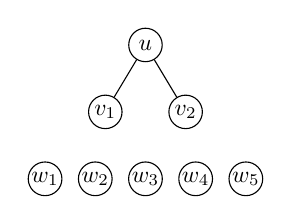
\begin{tikzpicture}[scale=0.85, every node/.style={scale=0.85,shape=circle,inner sep=.5pt,
                  minimum size=5mm}]
              \node[draw] (u) at (0,1) {$u$};
              \node[draw] (v1) at (-.6,0) {$v_1$};
              \node[draw] (v2) at (.6,0) {$v_2$};
              \node[draw] (w1) at (-1.5,-1) {$w_1$};
              \node[draw] (w2) at (-.75,-1) {$w_2$};
              \node[draw] (w3) at (0,-1) {$w_3$};
              \node[draw] (w4) at (.75,-1) {$w_4$};
              \node[draw] (w5) at (1.5,-1) {$w_5$};
              \draw (u) -- (v1);
              \draw (u) -- (v2);
          \end{tikzpicture}
        }
        \label{figure:gac-example-3}
    }
    \subfigure[][$H_2$] {
        \centering
        \scalebox{1}{
          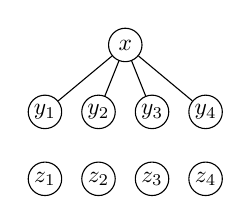
\begin{tikzpicture}[scale=0.85, every node/.style={scale=0.85,shape=circle,inner sep=.5pt,
                  minimum size=5mm}]
              \node[draw] (x) at (0,1) {$x$};
              \node[draw] (y1) at (-1.2,0) {$y_1$};
              \node[draw] (y2) at (-.4,0) {$y_2$};
              \node[draw] (y3) at (.4,0) {$y_3$};
              \node[draw] (y4) at (1.2,0) {$y_4$};
              \node[draw] (z1) at (-1.2,-1) {$z_1$};
              \node[draw] (z2) at (-.4,-1) {$z_2$};
              \node[draw] (z3) at (.4,-1) {$z_3$};
              \node[draw] (z4) at (1.2,-1) {$z_4$};
              \draw (x) -- (y1);
              \draw (x) -- (y2);
              \draw (x) -- (y3);
              \draw (x) -- (y4);
          \end{tikzpicture}
        }
        \label{figure:gac-example-4}
    }
    \subfigure[][$G_k$] {
        \centering
        \scalebox{1}{
          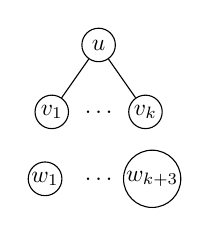
\begin{tikzpicture}[scale=0.85, every node/.style={scale=0.85,shape=circle,inner sep=.5pt,
                  minimum size=5mm}]
              \node[draw] (u) at (0,1) {$u$};
              \node[draw] (v1) at (-.7,0) {$v_1$};
              \node[] (vdots) at (0,0) {$\dots$};
              \node[draw] (v2) at (.7,0) {$v_k$};
              \node[draw] (w1) at (-.8,-1) {$w_1$};
              \node[] (wdots) at (0,-1) {$\dots$};
              \node[draw] (w5) at (.8,-1) {$w_{k+3}$};
              \draw (u) -- (v1);
              \draw (u) -- (v2);
          \end{tikzpicture}
        }
        \label{figure:gac-example-1}
    }
    \subfigure[][$H_k$] {
        \centering
        \scalebox{1}{
          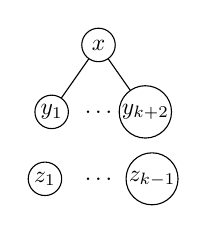
\begin{tikzpicture}[scale=0.85, every node/.style={scale=0.85,shape=circle,inner sep=.5pt,
                  minimum size=5mm}]
              \node[draw] (x) at (0,1) {$x$};
              \node[draw] (y1) at (-.7,0) {$y_1$};
              \node[] (ydots) at (0,0) {$\dots$};
              \node[draw] (y2) at (.7,0) {$y_{k+2}$};
              \node[draw] (z1) at (-.8,-1) {$z_1$};
              \node[] (zdots) at (0,-1) {$\dots$};
              \node[draw] (z5) at (.8,-1) {$z_{k-1}$};
              \draw (x) -- (y1);
              \draw (x) -- (y2);
          \end{tikzpicture}
        }
        \label{figure:gac-example-2}
    }
    \caption{Example graphs $G_2$ and $H_2$, and their generalised
    versions $G_k$ and $H_k$.}\label{figure:gac-example}
\end{figure}

When solving this instance, \McSplit-SI begins by mapping $u$ to $x$.  This leaves
two label classes:
$\langle \{v_1,v_2\}, \{y_1,y_2,y_3,y_4\} \rangle$
and
$\langle \{w_1,w_2,w_3,w_4,w_5\}, \{z_1,z_2,z_3,z_4\} \rangle$.  In the latter
label class, the set $V_G$ is larger than the set $V_H$, and therefore the
algorithm can backtrack and terminate.

Now we consider how the Glasgow algorithm behaves on this instance. After mapping
$u$ to $x$, the domains correspond to our label classes, as shown in the first two
columns of \Cref{tab:counting-all-diff}.  The remaining two columns of the table
illustrate the behaviour of the counting all-different propagator on these domains.
(Since all domains are of the same size, the stable sort function used by the algorithm
does not reorder the domains.)  The third column shows set $A$, which is the union
of domains in the current and previous rows.  The fourth column shows the number
of variables up to and including the current row.  Since $|A| \geq n$ on each row,
the propagator does not delete any values from the domains and does not conclude
that we can backtrack.

\begin{table}[h!]
\centering
\footnotesize
    \begin{tabular}{p{0.09\linewidth} p{0.16\linewidth} p{0.3\linewidth} p{0.08\linewidth}}
 \toprule
     Variable & Domain & $A$ & $n$\\ [0.5ex]
 \midrule
     $v_1$ & $\{y_1,y_2,y_3,y_4\}$ & $\{y_1,y_2,y_3,y_4\}$ & 1\\
     $v_2$ & $\{y_1,y_2,y_3,y_4\}$ & $\{y_1,y_2,y_3,y_4\}$ & 2\\
     $w_1$ & $\{z_1,z_2,z_3,z_4\}$ & $\{y_1,y_2,y_3,y_4,z_1,z_2,z_3,z_4\}$ & 3\\
     $w_2$ & $\{z_1,z_2,z_3,z_4\}$ & $\{y_1,y_2,y_3,y_4,z_1,z_2,z_3,z_4\}$ & 4\\
     $w_3$ & $\{z_1,z_2,z_3,z_4\}$ & $\{y_1,y_2,y_3,y_4,z_1,z_2,z_3,z_4\}$ & 5\\
     $w_4$ & $\{z_1,z_2,z_3,z_4\}$ & $\{y_1,y_2,y_3,y_4,z_1,z_2,z_3,z_4\}$ & 6\\
     $w_5$ & $\{z_1,z_2,z_3,z_4\}$ & $\{y_1,y_2,y_3,y_4,z_1,z_2,z_3,z_4\}$ & 7\\
%    $s_G$ & Pointer to Integer & Pointer to the first vertex of the $G$-set\\
%    \rule{0pt}{2.3ex}$e_G$ & Pointer to Integer & Pointer to one element past the last vertex of the $G$-set\\
 \bottomrule
\end{tabular}
\caption{A demonstration of the counting all-different propagator on $G_2$ and $H_2$
    after assigning $u$ to $x$.}
\label{tab:counting-all-diff}
\end{table}

The final two graphs in \Cref{figure:gac-example} generalise $G_2$ and $H_2$; as $k$ is incremented,
a vertex is added to each of the $v$, $w$, $y$ and $z$ sets.
\Cref{tab:gk-run-times} shows run times for the enumeration problem
using \McSplit-SI, Glasgow, and RI for a range of values of $k$.
VF3 was excluded from the experiment because the current version does not handle disconnected graphs correctly.
\McSplit-SI solves the instance $k=1\,000\,000$ in less than a second;
Glasgow and RI time out on the $k=10$ and $k=6$ instances respectively.

\begin{table}[h!]
\centering
\footnotesize
    \begin{tabular}{r r r r}
 \toprule
     $k$ & \McSplit-SI & Glasgow & RI \\ [0.5ex]
 \midrule
        3 & 0 & 0 & 2 \\
        4 & 0 & 0 & 84 \\
        5 & 0 & 2 & 3934 \\
        6 & 0 & 18 & * \\
        7 & 0 & 184 & * \\
        8 & 0 & 1849 & * \\
        9 & 0 & 21067 & * \\
        10 & 0 & * & * \\
        10000 & 5 & * & * \\
        100000 & 148 &  * & * \\
        1000000 & 584 & * & * \\
 \bottomrule
\end{tabular}
\caption{Run times in ms for the induced subgraph isomorphism enumeration problem on $G_k$.
    An asterisk indicates timeout at 30 seconds.}
\label{tab:gk-run-times}
\end{table}

\section{Experimental evaluation}

In this section, we compare the speed of \McSplit-SI with three state-of-the-art algorithms
on two sets of benchmark instances.  For the first set of instances, we solve the decision problem:
does there exist an induced subgraph isomorphism from the pattern graph to the target
graph?  For the second set of instances, we solve the problem of counting all induced subgraph
isomorphisms from the pattern to the target.

\subsection{Other solvers}

Our experiments compare \McSplit-SI with three state-of-the-art subgraph isomorphism solvers:
VF3, RI, and Glasgow.  

The Glasgow algorithm \cite{DBLP:conf/cp/McCreeshP15,DBLP:conf/gg/McCreeshP020}
was the fastest solver for hard induced subgraph isomorphism instances in a recent
experimental evaluation by Solnon \cite{DBLP:conf/gbrpr/Solnon19}.  The algorithm
uses a constraint programming approach, in which the domain of each vertex is represented
explicitly in memory.  Bitsets are used to represent domains and rows of each adjacency
matrix, allowing very fast updates to domains, particularly on dense graphs
\cite{ullmann1976algorithm}.  The Glasgow algorithm introduces the concept of
\emph{supplemental graphs}: graphs derived from the pattern and target graphs that
can also be used to filter domains.  This technique often results in a large
improvement to the solver's run time.  Unfortunately we cannot use the same technique
in \McSplit-SI because it breaks the invariant, required by \McSplit-SI's data structure,
that any two domains are either equal or disjoint.
We use the 14 March 2022 version of the Glasgow solver, published
online.\footnote{\url{https://github.com/ciaranm/glasgow-subgraph-solver}}

Like Glasgow, the VF3 \cite{DBLP:journals/pami/CarlettiFSV18} and RI
\cite{DBLP:journals/bmcbi/BonniciGPSF13,DBLP:journals/tcbb/BonniciG17}
solvers explore a search tree, adding one pair of vertices to the mapping at each
search node.  However, the data structures maintained by these algorithms are
much more lightweight than those of Glasgow.  VF3 and RI do not maintain
a domain for each vertex in the pattern graph; they simply store a partition
of the vertex set of each graph into three sets: ($A$) vertices that have been
mapped already, ($B$) unmapped vertices that are adjacent to at least one mapped vertex, and
($C$) all other unmapped vertices.
If the $B$ (resp. $C$) set of the target graph is smaller than the $B$ (resp. $C$)
set of the pattern graph, the algorithm can backtrack.
This data structure can be updated with the same
time complexity as the partitioning step of \McSplit-SI (and with a slightly
smaller constant factor given the simplicity of the data structure).  
However, its ability to prune the search tree is worse than that of \McSplit-SI
since the $B$ sets are a union of the label classes in \McSplit-SI, and it
leaves unavailable the smallest-domain-first heuristic used by \McSplit-SI.
(TODO mention RI-DS)
(TODO write about differences between VF3 and RI)

In terms of effort per search node, \McSplit-SI may be viewed intuitively as sitting
between Glasgow on one hand VF3 and RI on the other.

\subsection{Decision instances}

\subsection{Families of instances}

\subsection{Results}

\begin{figure}[h!]
    \centering
    \includegraphics*[width=0.7\textwidth]{14b-mcsplit-induced-si/decision-instances-experiment/experiment/plots/cumulative-with-disconnected-patterns-treated-as-timeout}
    \caption{cumulative-with-disconnected-patterns-treated-as-timeout}
    \label{figure:cumulative-with-disconnected-patterns-treated-as-timeout}
\end{figure}

\begin{figure}[h!]
    \centering
    \includegraphics*[width=0.7\textwidth]{14b-mcsplit-induced-si/decision-instances-experiment/experiment/plots/sat-cumulative-with-disconnected-patterns-treated-as-timeout}
    \caption{sat-cumulative-with-disconnected-patterns-treated-as-timeout}
    \label{figure:sat-cumulative-with-disconnected-patterns-treated-as-timeout}
\end{figure}

\begin{figure}[h!]
    \centering
    \includegraphics*[width=0.7\textwidth]{14b-mcsplit-induced-si/decision-instances-experiment/experiment/plots/unsat-cumulative-with-disconnected-patterns-treated-as-timeout}
    \caption{unsat-cumulative-with-disconnected-patterns-treated-as-timeout}
    \label{figure:unsat-cumulative-with-disconnected-patterns-treated-as-timeout}
\end{figure}

\begin{figure}[h!]
    \centering
    \includegraphics*[width=0.7\textwidth]{14b-mcsplit-induced-si/decision-instances-experiment/experiment/plots/cumulative-without-disconnected-pattern}
    \caption{cumulative-without-disconnected-pattern}
    \label{figure:cumulative-without-disconnected-pattern}
\end{figure}

\begin{figure}[h!]
    \centering
    \includegraphics*[width=0.45\textwidth]{14b-mcsplit-induced-si/decision-instances-experiment/experiment/plots/mcsplit-si-vs-adjmat}
    \caption{mcsplit-si-vs-adjmat}
    \label{figure:mcsplit-si-vs-adjmat}
\end{figure}

\begin{figure}[h!]
    \centering
    \includegraphics*[width=0.45\textwidth]{14b-mcsplit-induced-si/decision-instances-experiment/experiment/plots/mcsplit-si-vs-dom}
    \caption{mcsplit-si-vs-dom}
    \label{figure:mcsplit-si-vs-dom}
\end{figure}

\begin{figure}[h!]
    \centering
    \includegraphics*[width=0.45\textwidth]{14b-mcsplit-induced-si/decision-instances-experiment/experiment/plots/mcsplit-si-vs-glasgow}
    \caption{mcsplit-si-vs-glasgow}
    \label{figure:mcsplit-si-vs-glasgow}
\end{figure}

\begin{figure}[h!]
    \centering
    \includegraphics*[width=0.45\textwidth]{14b-mcsplit-induced-si/decision-instances-experiment/experiment/plots/mcsplit-si-vs-vf3}
    \caption{mcsplit-si-vs-vf3}
    \label{figure:mcsplit-si-vs-vf3}
\end{figure}

\subsection{Enumeration instances}

Our second set of benchmark instances is based on the MIVIA LDGraphs dataset
\cite{DBLP:journals/pami/CarlettiFSV18}.  In each LDGraphs instance, the pattern and
target graphs are random directed graphs with vertex labels but without edge labels.
Although the results of benchmarking graph algorithms on such instances cannot
always be extrapolated to real-world instances \cite{DBLP:conf/cp/McCreeshPST17},
we include these instances because they are the an established benchmark set,
and in particular they are the main set of instances used to demonstrate the
performance of VF3.

Rather than using the instance files provided by the authors of the MIVIA LDGraphs
dataset, we chose to generate our own random graphs from the same model and with the
same parameters.  We made this choice for two reasons: first, because of the large size
of the LDGraphs files (90 GBytes compressed), and second, so that we could add sparser
instances to the set of instances.

In each instance, both the pattern and target graph are generated using a directed-graph
version of the Erd\H{o}s-Rényi $G(n,p)$ model.  In this model, a graph on $n$ vertices
is generated, and each of the $n(n-1)$ possible directed edges is added with independent
probability $p$.  Carletti et al.\ use the values $\{0.2, 0.3, 0.4\}$ for $p$. In our experiment
we additionally use the values $0.05$ and $0.1$.

Following Carletti et al., we generate two families of directed graphs: an unlabelled family
and a family with no edge labels in which the vertex labels are chosen uniformly at random
from the set $\{1,\dots,8\}$.  (Carletti et al.\ generated a third family, in which labels
are chosen from a non-uniform distribution.  Their experimental results show very similar
outcomes for the uniform and non-uniform families, and therefore we have omitted the non-uniform
family from our experiment.)

For each value of $p$, we use the values
of $n$ for the target graph that were used by Carletti et al.; these are shown in \Cref{tab:carletti-n}.
In each instance, a randomly-selected subset of $20\%$ of the target vertices is selected,
and the subgraph induced by this subset is used as the pattern graph.

\FloatBarrier

\begin{table}[h!]
\centering
\footnotesize
 \begin{tabular}{p{0.2\linewidth} p{0.35\linewidth} p{0.35\linewidth}}
 \toprule
     $p$ & Target graph $n$ (unlabelled) & Target graph $n$ (labelled) \\ [0.5ex]
 \midrule
     $0.05$, $0.01$, and $0.2$ &
         300, 500, 750, 1000, 1250, 1500, 2000, 2500, 3000, 3500, 4000, 4500, 5000 &
         300, 500, 750, 1000, 1250, 1500, 2000, 2500, 3000, 3500, 4000, 4500, 5000,
         5500, 6000, 6500, 7000, 7500, 8000, 9000, 10000\\
     \rule{0pt}{2.3ex}$0.3$ & 
        300, 500, 750, 1000, 1250, 1500, 2000, 2500, 3000 &
        300, 500, 750, 1000, 1250, 1500, 2000, 2500, 3000, 3500, 4000, 4500, 5000,
        5500, 6000, 6500, 7000, 7500, 8000, 9000 \\
     \rule{0pt}{2.3ex}$0.4$ & 300, 500, 750, 1000, 1250, 1500 &
        300, 500, 750, 1000, 1250, 1500, 2000, 2500, 3000, 3500, 4000, 4500, 5000, 5500, 6000, 6500, 7000 \\
 \bottomrule
\end{tabular}
\caption{Values of $n$ used in enumeration instances}
\label{tab:carletti-n}
\end{table}

\FloatBarrier

\subsection{Results for unlabelled instances}

Each point shows the average of run times for 5 (?) instances.  The time limit was set at 1000 seconds, are timeouts are treated as 1000 seconds.  (Maybe there's a better way of presenting results with timeouts? A table?)

\begin{figure}[h!]
    \centering
    \includegraphics*[width=0.6\textwidth]{14b-mcsplit-induced-si/vf3-instances-experiment/experiment/plots/runtimes0.05-1.pdf}
    \caption{Run times on enumeration instances with random directed pattern and target graphs, $p=0.05$}
    \label{figure:TODO}
\end{figure}

\begin{figure}[h!]
    \centering
    \includegraphics*[width=0.6\textwidth]{14b-mcsplit-induced-si/vf3-instances-experiment/experiment/plots/runtimes0.1-1.pdf}
    \caption{Run times on enumeration instances with random directed pattern and target graphs, $p=0.1$}
    \label{figure:TODO}
\end{figure}

\begin{figure}[h!]
    \centering
    \includegraphics*[width=0.6\textwidth]{14b-mcsplit-induced-si/vf3-instances-experiment/experiment/plots/runtimes0.2-1.pdf}
    \caption{Run times on enumeration instances with random directed pattern and target graphs, $p=0.2$}
    \label{figure:TODO}
\end{figure}

\begin{figure}[h!]
    \centering
    \includegraphics*[width=0.6\textwidth]{14b-mcsplit-induced-si/vf3-instances-experiment/experiment/plots/runtimes0.3-1.pdf}
    \caption{Run times on enumeration instances with random directed pattern and target graphs, $p=0.3$}
    \label{figure:TODO}
\end{figure}

\begin{figure}[h!]
    \centering
    \includegraphics*[width=0.6\textwidth]{14b-mcsplit-induced-si/vf3-instances-experiment/experiment/plots/runtimes0.4-1.pdf}
    \caption{Run times on enumeration instances with random directed pattern and target graphs, $p=0.4$}
    \label{figure:TODO}
\end{figure}

\FloatBarrier

\subsection{Results for vertex-labelled instances}

\begin{figure}[h!]
    \centering
    \includegraphics*[width=0.6\textwidth]{14b-mcsplit-induced-si/vf3-instances-experiment/experiment/plots/runtimes0.05-1.pdf}
    \caption{Run times on enumeration instances with random directed pattern and target graphs, $p=0.05$}
    \label{figure:TODO}
\end{figure}

\begin{figure}[h!]
    \centering
    \includegraphics*[width=0.6\textwidth]{14b-mcsplit-induced-si/vf3-instances-experiment/experiment/plots/runtimes0.1-1.pdf}
    \caption{Run times on enumeration instances with random directed pattern and target graphs, $p=0.1$}
    \label{figure:TODO}
\end{figure}

\begin{figure}[h!]
    \centering
    \includegraphics*[width=0.6\textwidth]{14b-mcsplit-induced-si/vf3-instances-experiment/experiment/plots/runtimes0.2-1.pdf}
    \caption{Run times on enumeration instances with random directed pattern and target graphs, $p=0.2$}
    \label{figure:TODO}
\end{figure}

\begin{figure}[h!]
    \centering
    \includegraphics*[width=0.6\textwidth]{14b-mcsplit-induced-si/vf3-instances-experiment/experiment/plots/runtimes0.3-1.pdf}
    \caption{Run times on enumeration instances with random directed pattern and target graphs, $p=0.3$}
    \label{figure:TODO}
\end{figure}

\begin{figure}[h!]
    \centering
    \includegraphics*[width=0.6\textwidth]{14b-mcsplit-induced-si/vf3-instances-experiment/experiment/plots/runtimes0.4-1.pdf}
    \caption{Run times on enumeration instances with random directed pattern and target graphs, $p=0.4$}
    \label{figure:TODO}
\end{figure}

\FloatBarrier

\section{Conclusion}

We have introduced a version of McSplit for the induced subgraph isomorphism problem that is time- and memory-efficient for large, sparse graphs, and shown experimentally that it outperforms state-of-the-art algorithms on many instances.

Future work could use the data structures of McSplit-SI in the McSplit algorithm for maximum common induced subgraph.
